\documentclass[12pt,a4paper]{article}
\usepackage[utf8]{inputenc}
\usepackage{amsmath}
\usepackage{amsfonts}
\usepackage{amssymb}
\usepackage{graphicx}
\usepackage{hyperref}
\setlength{\parindent}{0em}
\setlength{\parskip}{1em}
\begin{document}

\section{Introduction}
The whole project will be divided into 3 parts:

\begin{itemize}
	\item Front end, including all the pages and client logic functions.
	\item Back end, including all the server logic functions.
	\item Marker.
\end{itemize}

Front end languages we will use are HTML, CSS and Javascript. The first two are pretty easy to learn because actually these two cannot be considered as \textbf{programming languages}. The main problem here is Javascript. This is mainly because it is too flexible to use especially when used in a collaborative project. It will become harder to debug while the project is getting larger. However at the beginning writing Javascript won't be a problem for you given all of you can write Python very well. I will talk about the details of writing Javascript in \textbf{How To Do} section.

Back end are the easiest part in our project because we don't need to providing many functions for users. As we chose Django as the web framework, we don't need to take much care about database. Another issue in back end is configuring all the applications running on server. This requires shell programming skill and quick-learning.

Marker is the core of this project. We need to overcome several problems to fully implement a good marker:
\begin{itemize}
	\item Code style checker (Partially Done)
	\item Test case checker (Partially Done)
	\item Sandbox
	\item Task queue
	\item Communication
\end{itemize} 

The first two have been partially implemented but haven't been fully tested yet. Sandbox and Task queue can secure our server. We need to decide how to communicate with back end in communication module.

\section{What To Learn}
\subsection{Languages}
\begin{itemize}
	\item HTML. (\href{http://www.w3schools.com/html/default.asp}{click to learn})
	\item CSS. (\href{http://www.w3schools.com/css/default.asp}{click to learn})
	\item Javascript. (\href{http://www.w3schools.com/js/default.asp}{click to learn})
	\item Python.
	\item Shell. (at least can understand and modify others' codes)
	\item SQL. (at least can understand others's codes)
\end{itemize}

\subsection{Frameworks}

In front end, we will use \href{http://getbootstrap.com/}{Bootstrap} as CSS framework and \href{https://jquery.com/}{JQuery} as the tool to get elements in HTML and communicating with back end using Ajax. (\href{http://getbootstrap.com/getting-started/}{click to learn Bootstrap}, \href{http://www.w3schools.com/jquery/default.asp}{click to learn JQuery})

In back end, we will use \href{https://www.djangoproject.com/}{Django}. Django provides URL routing, template and database model functions for us. I will provide a barebone project for you to fast start to code with Django.

\subsection{Tools and Applications}

\begin{itemize}
	\item \href{https://www.mysql.com/}{MySQL}. We will use MySql as database on server.
	\item \href{https://www.nginx.com/}{Nginx}. We will use Nginx as web server.
	\item \href{https://about.gitlab.com/}{GitLab}. This will be used as our private git repo and issue tracker.
	\item Git. Used as our version control system and collaboration system.
	\item IDE or editor. I suggest to choose \href{https://www.sublimetext.com/}{Sublime Text} or \href{https://www.jetbrains.com/pycharm/}{PyCharm}. You can use PyCharm for free using your student email.
\end{itemize}

\section{How To Do}
In order to give you a brief understanding of how the project works, I wrote a figure of how data flows between different parts.

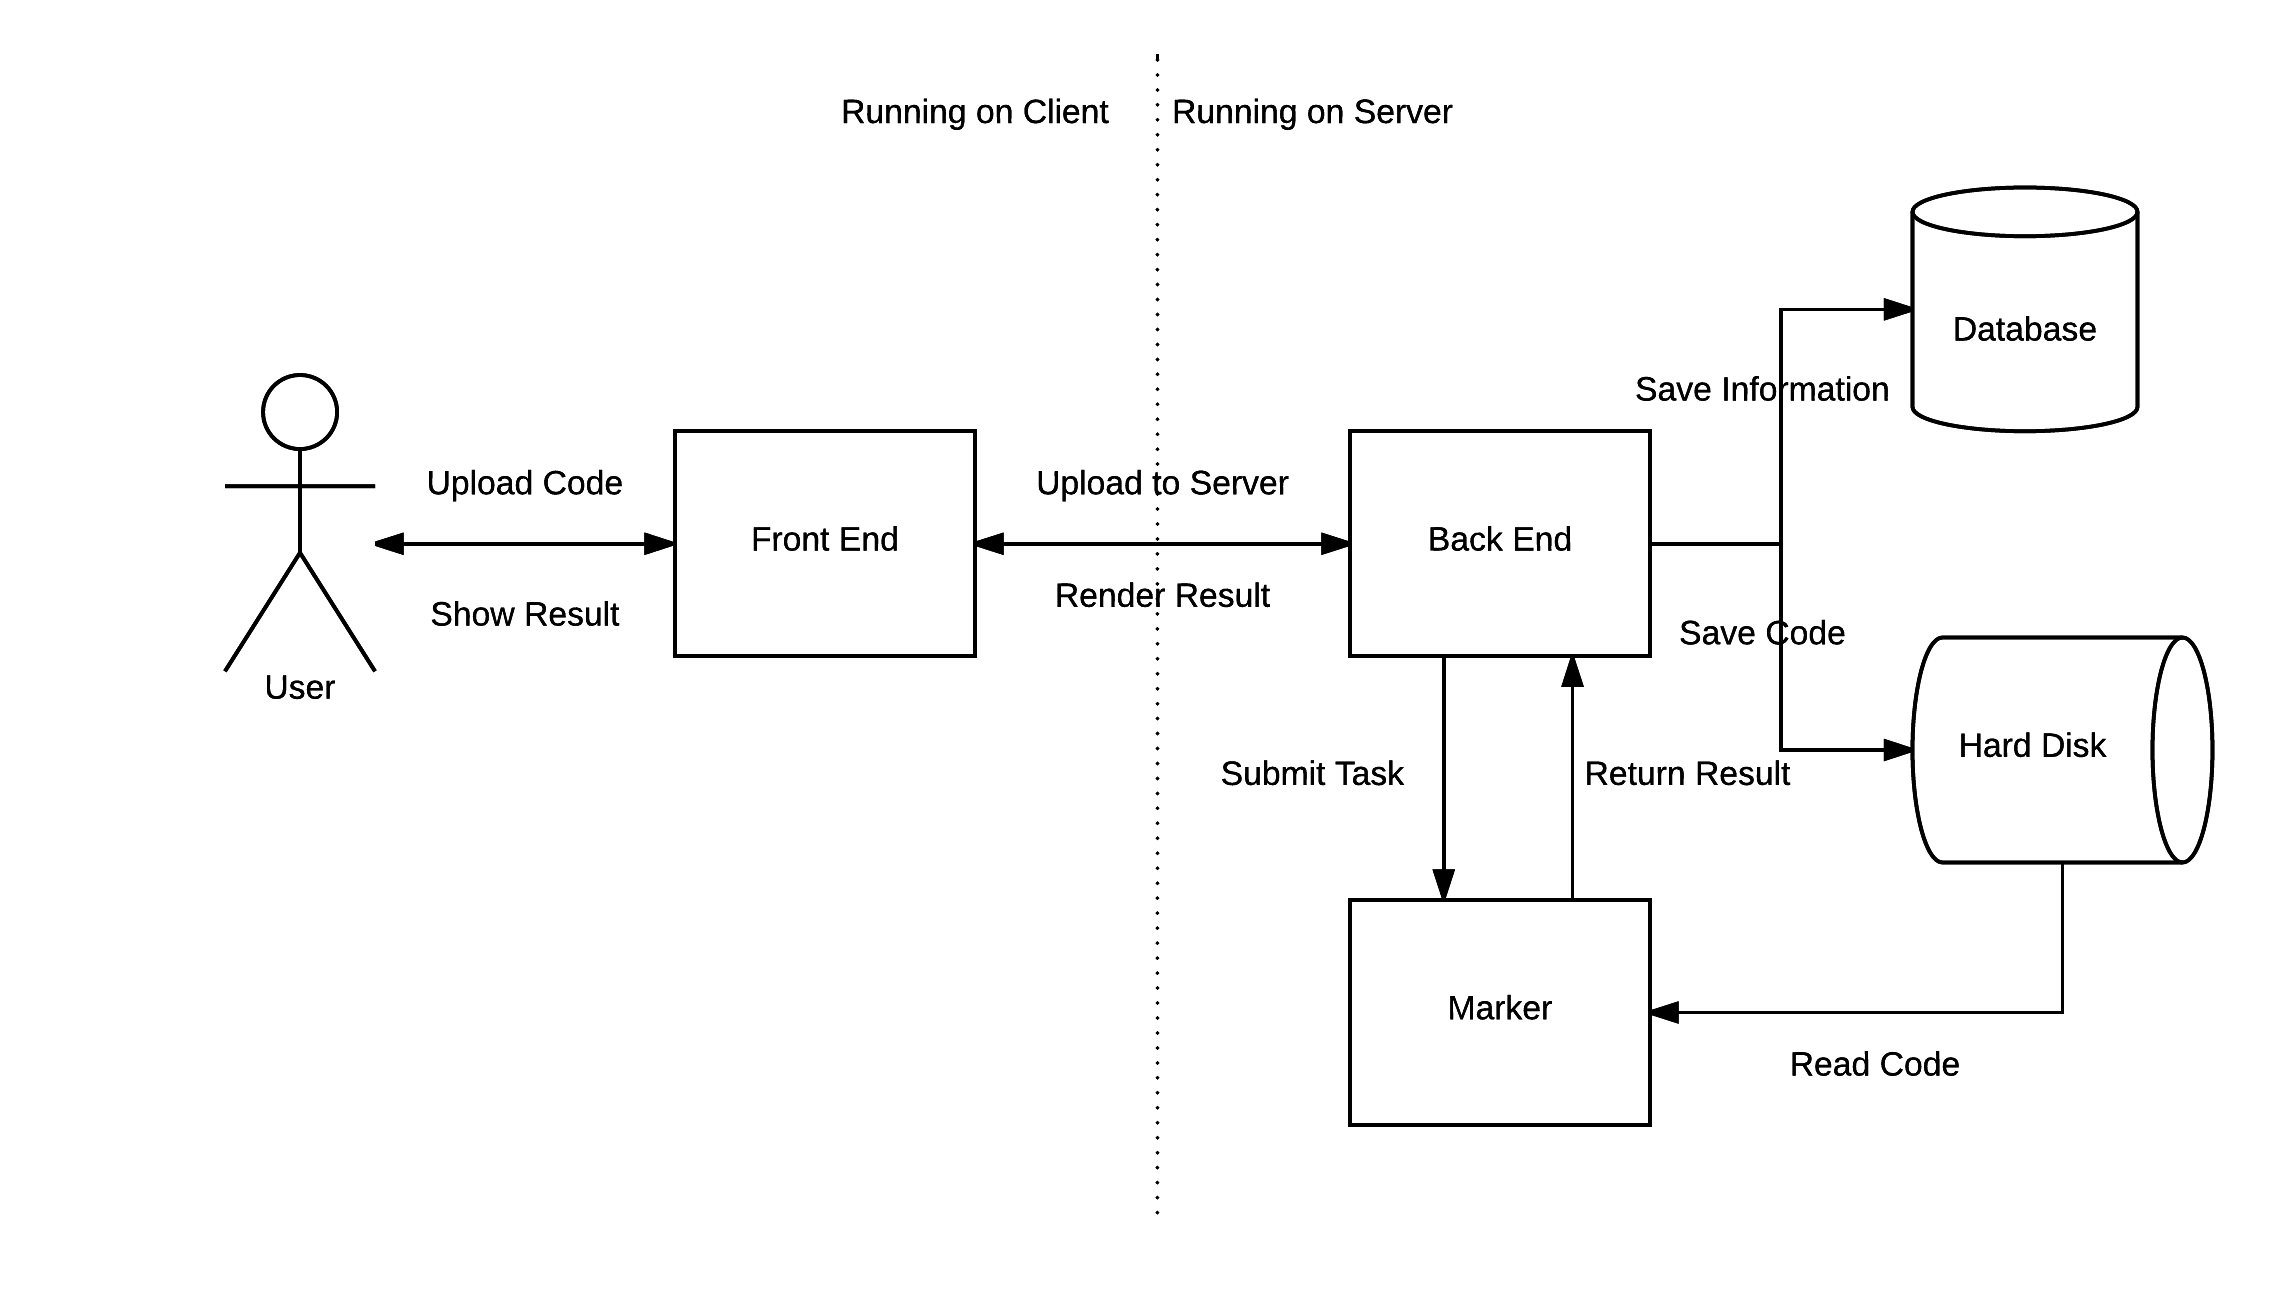
\includegraphics[scale=0.7]{flow-diagram.png}

After user submits his code, front end will upload the code to back end. And then back end saves the information of this submission into database and the code into hard disk. After saving, back end will submit a new code marking task to marker and then waiting for the code checking report. Once checking report is received, back end will render the result and send it back to front end.

So we can simply divide the whole project into these 3 parts and assign these sub-projects to each of you. I listed the details of tasks in each sub-projects here.

\subsection{Tasks}
\begin{itemize}
	\item List user cases. Write a document describing fully details of how user will use our project. 
	\item Front end
	\begin{itemize}
		\item Design pages
		\begin{itemize}
			\item Index Page, including several information of us and links to courses.
			\item Course Page
			\item Assignment Page
			\item Code Submit Page
			\item Result Page
		\end{itemize}
		Some of these pages may be merged into a single page and use Ajax to communicate with back end. First try to list all the functions provided for users on each page based on user case document and then list all the elements on each page. Then you can either draw prototypes or implement pages in a simple way. After this step finishes, we will hold a meeting to talk about which part should be improved.
		\item Implement pages. Once all of these have been done, implement pages using Django Template module, Bootstrap and JQuery. While implementing, write the protocol document to let back end know what should be given during rendering templates and Ajax.
		\item Test pages. Because our project now is simple enough, we can test the pages by hand. We will try to introduce some web testing framework after I come back.
	\end{itemize}
	
	\item Back end
	\begin{itemize}
		\item Install and configure all the applications running on server.
		\item Design modules
		\begin{itemize}
			\item Design all the view functions and models based on user case document.
			\item Finish protocol document with front end.
		\end{itemize}
		\item Implement modules.
		\item Test modules
		\begin{itemize}
			\item Unit testing should be finished during implementing. We can just use Django test module to test our functions.
			\item Integration testing will be done after complete implementing modules.
		\end{itemize}
	\end{itemize}
	
	\item Marker
	\begin{itemize}
		\item Read my code and test my code. 
		\item Implement a task queue and communicating API.
		\item Implement API for writing test cases of assignments in future.
	\end{itemize}
\end{itemize}

\subsection{Code Conventions}
\begin{itemize}
	\item \href{https://google.github.io/styleguide/pyguide.html}{Python code convention}
	\item \href{https://google.github.io/styleguide/javascriptguide.xml}{Javascript code convention}
\end{itemize}

\subsection{Workflow}
Read \href{https://www.atlassian.com/git/tutorials/syncing}{all the articles under Collaborating}. This workflow will be done in your daily developing. 

After a new feature has been submitted into master branch, someone should check master branch out on server. 

I wrote a gantt diagram to show the sequence of tasks.

\centering
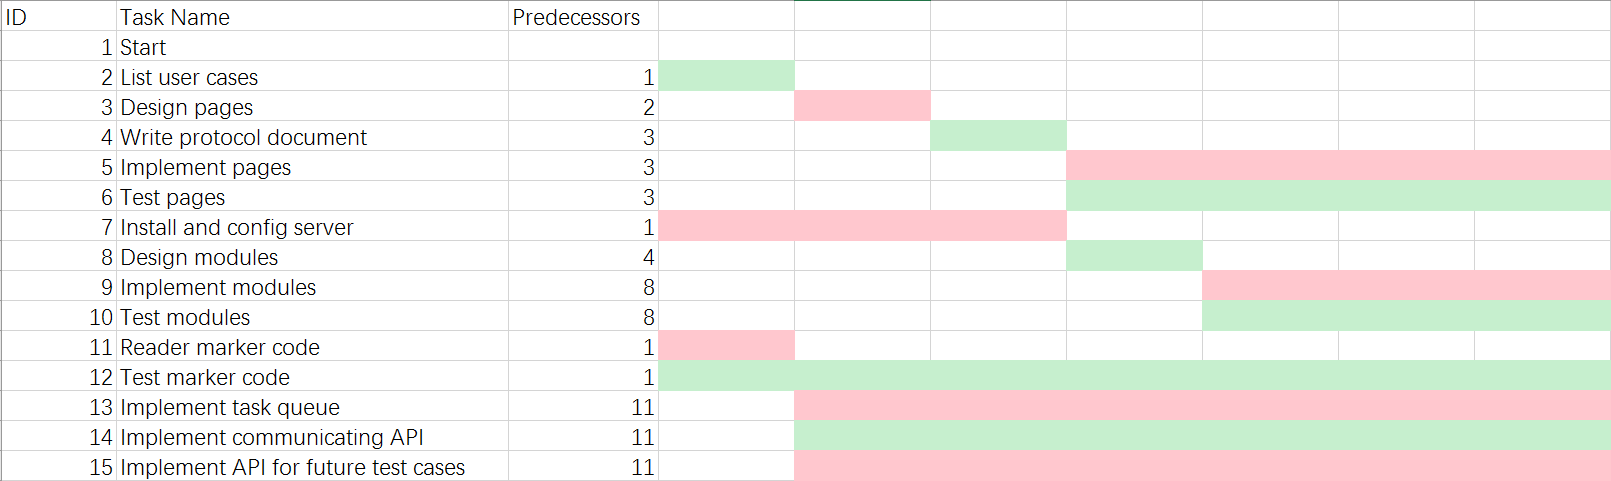
\includegraphics[scale=0.3]{gantt-diagram.png}
\end{document}